\documentclass[draft=false
              ,paper=a4
              ,twoside=false
              ,fontsize=11pt
              ,headsepline
              ,BCOR=10mm
              ]{scrbook}
\usepackage[ngerman,english]{babel}
%% see http://www.tex.ac.uk/cgi-bin/texfaq2html?label=uselmfonts
\usepackage[T1]{fontenc}
\usepackage[utf8]{inputenc}
\usepackage{libertine}
\usepackage{pifont}
\usepackage{microtype}
\usepackage{textcomp}
\usepackage[german,refpage]{nomencl}
\usepackage[ngerman,colorlinks=true]{hyperref}
\usepackage{setspace}
\usepackage{makeidx}
\usepackage{listings}
\usepackage{csquotes}
\usepackage{tikz}
\usepackage[
    backend=biber,
    style=ieee,
    sorting=nyt,
]{biblatex}
\addbibresource{literature.bib}
\usepackage{soul}
\usepackage{hawstyle}
\usepackage{scrhack}
\usepackage{subfiles}
\usepackage{graphicx}
\usepackage{float}
\usepackage{parskip}

%% define some colors
\colorlet{BackgroundColor}{gray!20}
\colorlet{KeywordColor}{blue}
\colorlet{CommentColor}{black!60}
%% for tables
\colorlet{HeadColor}{gray!60}
\colorlet{Color1}{blue!10}
\colorlet{Color2}{white}

%% configure colors
\HAWifprinter{
  \colorlet{BackgroundColor}{gray!20}
  \colorlet{KeywordColor}{black}
  \colorlet{CommentColor}{gray}
  % for tables
  \colorlet{HeadColor}{gray!60}
  \colorlet{Color1}{gray!40}
  \colorlet{Color2}{white}
}{}
\lstset{
  language=Java,
  numbers=left,
  numberstyle=\tiny,
  stepnumber=1,
  numbersep=5pt,
  basicstyle=\ttfamily\small,
  keywordstyle=\color{KeywordColor}\bfseries,
  identifierstyle=\color{black},
  commentstyle=\color{CommentColor},
  backgroundcolor=\color{BackgroundColor},
  captionpos=b,
  fontadjust=true
}
\lstset{escapeinside={(*@}{@*)}, % used to enter latex code inside listings
        morekeywords={uint32_t, int32_t}
}
\ifpdfoutput{
  \hypersetup{bookmarksopen=false,bookmarksnumbered,linktocpage}
}{}

%% more fancy C++
\DeclareRobustCommand{\cxx}{C\raisebox{0.25ex}{{\scriptsize +\kern-0.25ex +}}}

\clubpenalty=10000
\widowpenalty=10000
\displaywidowpenalty=10000
\setcounter{secnumdepth}{3}

% unknown hyphenations
\hyphenation{
}

%% recalculate text area
\typearea[current]{last}

\makeindex
\makenomenclature

\begin{document}
\selectlanguage{ngerman}

%%%%%
%% customize (see readme.pdf for supported values)
\HAWThesisProperties{Author={Dennis Schröder}
                    ,Title={\textit{Agentenorientierte Softwareentwicklung} im Kontext der \textit{Multi-Roboter-Wegplanung}}
                    ,EnglishTitle={\textit{Agent-oriented software engineering} in the context of \textit{mutli-robot path planning}}
                    ,ThesisType={Bachelorarbeit}
                    ,ExaminationType={Bachelorprüfung}
                    ,DegreeProgramme={Bachelor of Science Technische Informatik}
                    ,ThesisExperts={Prof. Dr. Martin Becke \and Prof. Dr.-Ing. Andreas Meisel}
                    ,ReleaseDate={1. April 2019}
                  }

%% title
\frontmatter

%% output title page
\maketitle

\onehalfspacing

%% add abstract pages
\HAWAbstractPage
{Agentenorientierte Softwareentwicklung, AoSE, Multi-Roboter-Wegplanung, Agenten, JADE, CoDy Algorithmus, Smart Chair, CaDS}
{\textit{Internet of Things} (IoT), \textit{Ubiquitous Computing} und \textit{Industrie 4.0} sind Begriffe, die in letzter Zeit immer mehr an Bedeutung gewinnen. Gemeinsam haben diese Themengebiete vor allem ihren Fokus auf der Vernetzung von Rechnern. Die Anforderung an die Skalierbarkeit solcher Systeme wird mit der Anzahl der Geräte und dem Grad der Vernetzung steigen und somit zukünftig immer wichtiger werden. Auch mit dem Blick auf das Jahr 2022, in dem 50 Milliarden IoT-Geräte aktiv sein sollen.\newline
Im Rahmen dieser Bachelorarbeit wird ein solches skalierendes System entwickelt. Eine Kernanforderung an das System ist es, mit unterschiedlichen Anzahlen von Teilnehmern souverän umgehen zu können. Die Spanne reicht von wenigen Einzelnen bis vielen Hunderten. Um diesen Grad der Skalierbarkeit zu erreichen, wird das System mit Hilfe der \textit{agentenorientierten Softwareenticklung} (AoSE) umgesetzt. Als Produkt entsteht ein Multi-Agenten-System, das durch das \textit{Java Agent Development Framework} (JADE) implementiert wird. Zusammen mit dem \textit{Cooperative Dynamic} (CoDy)-Algorithmus entsteht ein kooperatives System aus Agenten die sich in einer zweidimensionalen \textit{Gridworld} bewegen können.\newline
Denn das Projekt, an dem die Skalierbarkeit des AoSE-Ansatzes aufgezeigt wird, beschäftigt sich mit der Erweiterung der \textit{Smart Chairs} der \textit{Communication and Distributed System} (CaDS)-Arbeitsgruppe der \textit{Hochschule für angewandte Wissenschaften Hamburg}, um die Fähigkeit an bestimmte Plätze fahren zu können.\newline
In einer selbst entwickelten Simulationsumgebung werden dann Experimente aus \cite{book:regele} wiederholt. Anhand der Ergebnisse, den zuvor definierten qualitativen Merkmalen und Anforderungen sowie den Kerneigenschaften des Multi-Agenten-Systems, Dezentralität und Autonomie, wird dann die Skalierbarkeit diskutiert und das Projekt bewertet.}
{Agent-oriented software engineering, AoSE, Mutli-robot path planning, Agents, JADE, CoDy Algorithm, Smart Chair, CaDS}
{\textit{Internet of Things} (IoT), \textit{ubiquitous computing} and \textit{Industry 4.0} are terms that are gaining importance lately. These topics share a focus on more complex networked computers. The scalability requirement of such systems will increase with the number of devices and the degree of networking and thus become more important in the future. Experts estimate that in the year 2022 that 50 billion IoT devices will be active.\newline
Such a scaling system will be developed within the scope of this bachelor thesis. A core requirement of the system is to handle different numbers of participants confidently. The range varies from a few to many hundreds individuals. To achieve this level of scalability, the system is implemented using \textit{agent-oriented software engineering} (AoSE). The product is a multi-agent system, which is implemented with the \textit{Java Agent Development Framework} (JADE). Together with the \textit{Cooperative Dynamic} (CoDy) algorithm, it creates a cooperative system of agents that can move in a two-dimensional \textit{gridworld}.\newline
The project, which demonstrates the scalability of the AoSE approach, addresses the extension of the \textit{Smart Chairs} of the \textit{Communication and Distributed System} (CaDS) team from the \textit{Hamburg University of Applied Sciences} to be able to drive to certain places.\newline
Experiments from \cite{book:regele} will be repeated in a self developed simulator. Based on the results, the previously defined qualitative characteristics and requirements as well as the core properties of the multi-agent system, decentralization and autonomy, the scalability is discussed and the project evaluated.}

\newpage
\singlespacing

\setcounter{tocdepth}{3}
\tableofcontents
\newpage
%% enable if these lists should be shown on their own page
\listoftables
\listoffigures
\lstlistoflistings

%% main
\mainmatter
\onehalfspacing

%%%%%% Chapters
\chapter{Einleitung}
%
\section{Motivation}
\label{chap:motivation}
Die \textit{Communication and Distributed System} (CaDS)-Arbeitsgruppe der \textit{Hochschule für angewandte Wissenschaften} (HAW) präsentiert ihre \textit{Smart Chairs}\footnote{Ein Bürostuhl, der mit verschiedenen (Druck-, Abstands- und Temperatur-) Sensoren \cite{web:smartChair}) sowie einem Antrieb ausgestattet ist.} auf Veranstaltungen, um Aufmerksamkeit für sich und die HAW zu generieren. In erster Linie werden die \textit{Smart Chairs} als IoT-Geräte betrachtet und dienen der Erforschung dieses Themengebiets.\newline
Die CaDS-Arbeitsgruppe möchte, dass die \textit{Smart Chairs} sich autonom bewegen, um eine Funktion für den kürzlich hinzugefügten Antrieb zu haben. Dabei sollen die \textit{Smart Chairs} bestimmte Positionen in einem Raum anfahren, um einen realen Anwendungsfall darstellen zu können. Dies könnte zum Beispiel das Fahren an Schreibtische sein. Je näher man einem realem beziehungsweise alltäglichem Szenario ist, desto interessanter und greifbarer wirkt die Anwendung.Diese grobe Definition wird im Rahmen dieser Arbeit nicht weiter vertieft, da der Fokus im Entwickeln eines \textit{Proof of Concepts} (PoC) liegt und hierfür ein detailliert ausformulierter Anwendungsfall nicht erforderlich ist. Lediglich die groben Rahmenbedingungen müssen bekannt sein, welche im folgenden Kapitel festgehalten werden.
%
\section{Anforderungen}
\label{chap:anforderungen}
In diesem Kapitel werden die Anforderungen an den Anwendungsfall beziehungsweise an das Softwaresystem aufgezählt.\newline
\begin{enumerate}
\item \textbf{Skalierbarkeit} ist eine wichtige Anforderung an das System, da der Anwendungsfall die Anzahl der Teilnehmer nicht klar vorgibt. Das System soll also skalieren, um mit einem einzigen sowie auch mit mehreren Teilnehmern umgehen können.
\item Das System soll \textbf{robust} sein. Die Positionen, die die \textit{Smart Chairs} anfahren, sollen, wenn sie erreicht werden können, in endlicher Zeit erreicht werden. Dabei müssen die Wege nicht optimal bezüglich ihrer Zeit oder Strecke gewählt werden.
\item Das System soll in \textbf{Echtzeit} agieren. Damit soll vermieden werden, dass lange Pausen oder Initialisierungsphasen eintreten.
\item Das System soll mit Hilfe von AoSE umgesetzt werden. Die \textit{Smart Chairs} sollen jeweils als \textbf{Agent} abgebildet werden.
\item Das System soll Hindernisse erkennen und ihnen ausweichen. Es soll also \textbf{nicht} zu \textbf{Kollisionen} kommen.
\end{enumerate}
Zwar sind alle Anforderungen wichtig, sie können, im Rahmen dieser Arbeit, aber nicht alle mit gleichem Gewicht bearbeitet werden. Der Fokus liegt auf der Skalierbarkeit und dem AoSE, da sie Teile der Forschungsfrage sind.
%
\section{Kapitelkurzzusammenfassungen}
\label{chap:kapitel}
% Diese Arbeit gliedert sich in folgende weitere Kapitel.\newline\newline
% %
% Kapitel \hyperref[chap:theorie]{2} - Theoretischer Hintergrund - gibt einen Einblick in die Theorie verwendeter Methodiken, Konzepte und Algorithmen. Außerdem wird die Wahl der jeweiligen Methodiken, Konzepte und Algorithmen begründet und eine Auswahl an Alternativen dargestellt.\newline\newline
% %
% Kapitel \hyperref[chap:jadeDesign]{3}- Designen mit JADE -  beschreibt den allgemeinen Designprozess eines Multi-Agenten Systems unter der Anleitung von \textit{JADE}. Der Prozess wird an Beispielen explizit aufgezeigt.\newline\newline
% %
% Kapitel \hyperref[chap:methodik]{4} - Methodik - stellt die begründete Auswahl der Methode dar.\newline\newline
% %
% Kapitel \hyperref[chap:datenerhebung]{5} - Datenerhebung - beschreibt zum Einen die Simulationsumgebung und zum Anderen die Metriken, die in Kapitel 6 verwendet werden. Darüber hinaus wird die Strategie zur Validierung der Experimente erklärt.\newline\newline
% %
% Kapitel \hyperref[chap:experimente]{6} - Experimente - listet Experimente nach folgendem Schema auf: Fragestellung, Versuchsaufbau und Beobachtungen.\newline\newline
% %
% Kapitel \hyperref[chap:diskussion]{7} - Diskussion - diskutiert die Beobachtungen der Experimente im Hinblick auf die Fragestellung.\newline\newline
% %
% Kapitel \hyperref[chap:fazit]{8} - Fazit - fasst den Kern der Arbeit zusammen und gibt einen Ausblick.

TODO redo!
%
\label{chap:einleitung}
%
\chapter{Theoretischer Hintergrund}
\label{chap:theorie}
\section{Agentenorientierte Softwareentwicklung}
\label{chap:aose}
Ein Agent ist für die AoSE, dass was ein Objekt für die OOP ist. AoSE ist, so wie die OOP auch, ein Programmierparadigma. Um AoSE zu verstehen, wird folgend der Begriff des Agenten definiert.

\subsection{Agent}
\label{chap:aose_agent}
Es existiert keine universelle Definition für Agenten \cite{book:padgham}. Jedoch gibt es Eigenschaften die einen Agenten beschreiben, die von diversen Definitionen aufgegriffen werden. Ein Agent ist:
\begin{itemize}
\item \textbf{zielorientiert.} Er hat ein oder mehrere Ziele. Sein Verhalten ist darauf ausgelegt, diese zu erfüllen.
\item \textbf{autonom.} Ein Agent kontrolliert seinen internen Status und entscheidet selbständig, ob und welche Aktion er ausführt.
\item \textbf{reaktiv.} Auf Änderungen der Umwelt kann reagiert werden.
\item \textbf{proaktiv.} Der Agent ergreift Eigeninitiative. Es sind also keine Befehle von außen notwendig, um zu handeln.
\item \textbf{sozial.} Er interagiert "'menschenähnlich"' mit anderen Agenten. Das bedeutet, dass Agenten Verhandeln, Koordinieren, Kooperieren und so weiter.
\end{itemize}\cite{book:padgham}\cite{book:jade}\cite{article:flexibleSoftware}

Eingangs wurde der Vergleich mit OOP gemacht. Objekte und Agenten teilen sich tatsächlich viele Merkmale. Objekte kapseln ihre Identität und ihren Status. Sie kontrollieren aber nicht ihr Verhalten. Die Methoden der Objekte werden von außen und potenziell zu jeder Zeit aufgerufen. Agenten kapseln dies jedoch zusätzlich. Sie verfügen selbständig über ihre Methoden. Sie treten aber auch in komplexe Verhandlungen mit anderen Agenten. Zwar können die Konzepte des AoSE auch mit OOP implementieren, jedoch fehlen der OOP wichtige Konzepte. \cite{article:flexibleSoftware} Das Verhältnis von AoSE zur OOP ist so ähnlich, wie das Verhältnis zwischen der iterativen und der OOP. Weshalb die AoSE auch als nächster evolutionärer Schritt bezeichnet wird \cite{article:objectsVsAgents}.


Über die Zeit wurde es immer wichtiger lose Kopplung und hohe Kapselung in Software zu erreichen. AoSE führt diesen Trend konsequent weiter, indem eine Entität seinen eigen Kontrollfluss kontrolliert und damit seine Absichten kapselt. Diese Attribute gewinnen an Gewicht, je komplexer ein Softwaresystem ist. \cite{article:flexibleSoftware}.

In dieser Arbeit wird mit Hilfe der AoSE ein Multi-Agenten-System entwickelt.
%
\section{JADE}
\label{chap:jade}
Die \textit{Foundation for Intelligent Physical Agents} (FIPA) der \textit{IEEE Computer Society} hat im Bereich des Multi-Agenten-Systems mehrere Standards erarbeitet. Diese Standards beschreiben alle grundlegenden Elemente und Funktionen, die für eine Multi-Agenten-Plattform benötigt werden. \cite{article:flexibleSoftware}

Es gibt einige Projekte, die diesen Standard implementieren \cite{web:fipaList}. Unter diesen eignet sich das \textit{Java Agent Development Framework} (JADE) am besten für dieses Projekt. Zum einen ist das JADE Framwork in \textit{Java} implementiert und somit plattformunabhängig \cite{web:java}. Es ist open-source. Es kann also eigenständig verändert und erweitert werden. Zudem ist die Benutzung des Frameworks nicht mit Lizenzkosten verbunden. Zuletzt ist JADE in Form von \cite{book:jade} detailliert beschrieben.

In den folgenden Kapiteln wird eine Auswahl wichtiger Grundkonzepte des JADE Framworks vorgestellt. 

\subsection{Grundlagen}
\label{chap:jade_grundlagen}
\begin{figure}[H]
    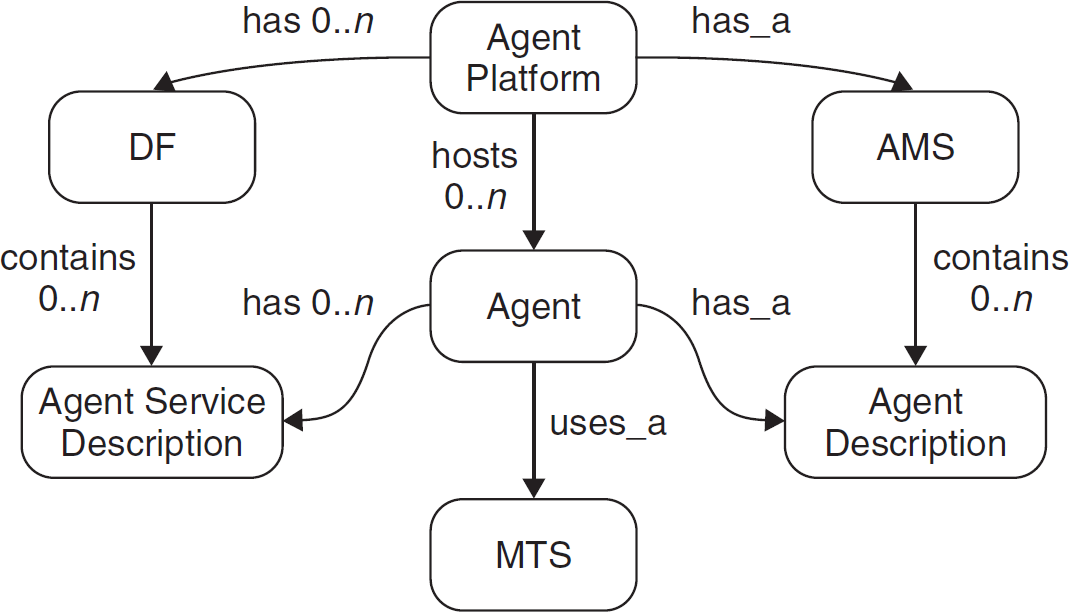
\includegraphics[width=10cm]{images/jade_structure.png}
    \centering
    \caption{\textit{Entity-Relationship}-Diagramm aus \cite{book:jade}}
    \label{fig:jade_structure}
\end{figure}

\paragraph{\textit{Agent Platform} (AP)}
Die AP beschreibt die physikalische Infrastruktur in der die Agenten ausgeführt werden. Hier sind die Rechner, die Netzwerke, die Betriebssysteme, das \textit{Agent Management System}, die Agenten selbst und zusätzliche Software mit inbegriffen.

\paragraph{Agent}
Ein Agent existiert in der AP und bietet ein oder mehrere Services die mit Hilfe einer \textit{Service Description} veröffentlicht sind. Ein Agent hat ein eindeutigen \textit{FIPA Agent Identifier} (AID).  

\paragraph{Diretory Faciliator (DF)}
Der DF ist eine optionale Komponente. Der DF stellt den Agenten einen "'Gelbe Seiten"'-Service zur Verfügung und hält eine komplette Liste aller Agenten. Der "'Gelbe Seiten"'-Service wird von den Agenten genutzt um ihre Services zu registrieren und somit den anderen Agenten verfügbar zu machen. Die AP kann beliebig viele DF starten, die ihre Daten untereinander synchronisieren.

\paragraph{Agent Management System (AMS)}
Das AMS ist für das Erstellen und Löschen der Agenten verantwortlich. Jeder Agent muss sich beim AMS registrieren. Bei diesem Schritt vergibt das AMS dann die AID für die Agenten. Ein Agent beendet sich, wenn er sich vom AMS abmeldet. Das AMS ist als eine Entität zu verstehen und erstreckt sich auch über mehrere Rechner.

\paragraph{Message Transport Service (MTS)} Dieser Service wird von der AP bereitgestellt. Über ihn können die Agenten Nachrichten austauschen.
%
\subsection{Behaviour}
\label{chap:jade_agent}
Ein \textit{Behaviour} ist eine Aufgabe die ein Agent ausführen kann und als erbende Klasse von \texttt{jade.core.behaviours.Behaviour} implementiert ist. Für jeden Agenten startet die JADE Umgebung einen Thread. Ein \textit{Behaviour} wird über einen Scheduler auf diesem Thread ausgeführt. Der Agent fügt ein \textit{Behaviour} mit \texttt{addBehaviour()} der Scheduling-Queue hinzu. Dies kann der Agent während der Initialisierungsphase in der \texttt{steup()} Methode tun oder innerhalb eines \textit{Behaviours}. Jede \textit{Behaviour}-Subklasse muss die \texttt{action()} und \texttt{done()} Methode implementieren. Die \texttt{action()} Methode enthält die Logik, also den auszuführenden Code, des \textit{Behaviours}. Die \texttt{done()} Methode gibt einen \texttt{boolean} zurück, der Aussage darüber trifft, ob das \textit{Behaviour} seine Aufgabe abgeschlossen hat und damit aus Scheduling-Queue entfernt werden soll. Ein Agent kann mehrere \textit{Behavoiur} ausführen. Ein \textit{Behavoiur} ist jedoch nicht preemptive. Wenn die \texttt{action()} Methode vom Scheduler aufgerufen wird, kann diese nicht unterbrochen werden. Das \textit{Behaviour} muss also selbständig diese Ressource wieder freigeben. \cite{book:jade}

Das JADE Framwork stellt jedoch nicht nur den Basistypen zur Verfügung, sondern implementiert weitere abstrakte \textit{Behaviour}. Folgend wird eine Auswahl aus \cite{book:jade} vorgestellt.

\paragraph{One-Shot Behaviour}
Für das \texttt{jade.core.behaviours.OneShotBehaviour} muss eine erbende Klasse nur die \texttt{action()} Methode implementieren. \texttt{done()} liefert standardmäßig \texttt{true} zurück. Ein \textit{One-Shot Berhaviour} wird also nur einmal ausgeführt.

\paragraph{Cyclic Behaviour}
Das \texttt{jade.core.behaviours.CyclicBehaviour} ist dem \textit{One-Shot Behaviour} recht ähnlich. Die \texttt{done()} Methode liefert jedoch standardmäßig \texttt{false} zurück. Ein \textit{Cyclic Behaviour} beendet sich also nie.

\paragraph{Ticker Behaviour}
Das \texttt{jade.core.behaviours.TickerBehaviour} implementiert sowohl \texttt{action()} als auch \texttt{done()} Methoden. Die \texttt{done()} Methode liefert immer \texttt{false} zurück. Die \texttt{action()} Methode führt die \texttt{onTick()} Methode periodisch aus. Das Zeitintervall wird über den Konstruktor definiert. Das \textit{Ticker Behavior} ist selbst eine abstrakte Klasse. Erbende Klassen implementieren die Methode \texttt{onTick()}.
%
\subsection{Kommunikation}
\label{chap:jade_kommunikation}
Agenten interagieren miteinander. Dies geschieht indirekt über das Verändern der Umwelt oder durch direkte Kommunikation. Die direkte Kommunikation ist wahrscheinlich eines des wichtigsten Funktionen des JADE Frameworks. Die Kommunikation zwischen Agenten erfolgt durch den asynchronen Nachrichtenaustausch. Jeder Agent besitzt eine Queue in der alle Nachrichten eines Agenten empfangen werden. Eine Nachricht hält dabei mehrere Felder:
\begin{itemize}
\item Die ID des \textbf{Senders}
\item Eine Liste, die alle \textbf{Empfänger} enthält.
\item Die \textbf{Absicht} der Nachricht. Die FIPA definiert hier eine Liste mit Möglichkeiten. Zum Beispiel "'Inform"'. Der Sender berichtet den Empfänger einen Fakt.
\item Den \textbf{Inhalt}, den der Sender mitteilen möchte.
\item Die \textbf{Kodierung} der Nachricht. So das die Empfänger wissen, wie die Nachricht zu lesen ist.
\end{itemize} \cite{book:jade}

%
\section{CoDy Algorithmus}
\label{chap:cody}
Ein Wegplanungs-Algorithmus kann entweder verteilt oder zentral arbeiten. Ein zentraler Algorithmus hat aber das Problem, dass der Berechnungsaufwand quadratisch von der Anzahl der Agenten abhängig ist (TODO Quelle). Ist für diese Arbeit also nicht interessant, da ein potentiell stark skalierendes Agenten-System zum Einsatz kommt. Ein echtzeitfähiger, verteilter und skalierender Algorithmus ist der \textit{CoDy Algorithmus}. Der CoDy Algorithmus berechnet die Wege für jeden Agenten aus Sicht der jeweiligen Agenten und löst mit Hilfe von heuristischer Prioritätsanpassung auftretende Konflikte. Der \textit{CoDy Algorithmus} hat bestimmte Voraussetzungen an das implementierende System. Es soll verteilt sein, muss den Agenten die Möglichkeit bieten, untereinander zu kommunizieren und homogen sein. Zusätzlich muss ein Agent in der Lage sein seine Umgebung zu erfassen, entweder durch die eigene Sensorik oder durch Kommunikation mit anderen Agenten. Alle Voraussetzungen können erfüllt werden. \cite{book:regele}

Die Funktionsweise des CoDy Algorithmus wird in den folgenden Unterkapiteln genauer beschrieben. Es soll aber nicht Sinn dieser Arbeit sein, die Dissertation wiederzugeben. Die grundlegenden Elemente und Funktionen werden nicht nur zum Grundverständnis wiedergegeben. Vor allem soll aber eine Basis geschaffen werden, auf deren Grund dann im Kapitel (TODO link) beschrieben werden kann, wie der Algorithmus umgesetzt wird und wo es zu Abweichungen kommt.
\subsection{Grundlagen}
\label{chap:grundlagen}
In diesem Kapitel werden die grundlegenden Mechanismen und Elemente des CoDy Algorithmus vorgestellt.

\subsubsection{Das Weltmodell}
\label{chap:weltmodell}
\input{chapter/theorie/cody/grundlagen/weltmodell.tex}
%
\subsubsection{Die Entfernungskarte}
\label{chap:entfernungskarte}
\input{chapter/theorie/cody/grundlagen/entfernungskarte.tex}
%
\subsubsection{Die Umgebungskarte}
\label{chap:umgebungskarte}
\input{chapter/theorie/cody/grundlagen/umgebungskarte.tex}
%
\subsubsection{Die Erreichbarkeitskarte}
\label{chap:erreichbarkeitskarte}
\input{chapter/theorie/cody/grundlagen/erreichbarkeitskarte.tex}
%
\subsubsection{Der Raum-Zeit-Pfad}
\label{chap:raum-zeit-pfad}
\input{chapter/theorie/cody/grundlagen/raum-zeit-pfad.tex}

%
\subsection{Konfliktverarbeitung}
\label{chap:konfliktverarbeitung}
Die Agenten des \textit{CoDy Algorithmus} sind kooperativ. Sie sind also in der Lage die eigenen "'Bedürfnisse"' zurückzustellen. Man kann zwischen passiver und aktiver Kooperation unterscheiden. Bei der aktiven Kooperation kann ein Agent die Planung übernehmen und bei anderen Agenten nach Zustimmung oder Ablehnung fragen. Bei der passiven Kooperation müssen alle in einem Konflikt beteiligten Agenten die gesamte Situation berechnen und dann anschließend in einer Verhandlung ihre Lösungen diskutieren. Die passive Kooperation hat gegenüber der aktiven Kooperation vor allem den Vorteil, dass der Kommunikationsaufwand deutlich geringer ist. Sie ist aber auch robuster und der Berechnungsaufwand, so wie sie im CoDy Algorithmus umgesetzt ist, geringer. Die echte passive Kooperation kann sehr ineffizient sein. Deshalb benutzt der CoDy Algorithmus eine abgewandelte Form. Agenten, die potenziell in einen Konflikt geraten können, kommunizieren in einer festen Reihenfolge (siehe Kapitel \ref{chap:kommunikation}) und planen nur ihre eigenen Wege. \cite{book:regele}\newline Folgende Beispielsituation:
Agent "'0"' überschreibt einen Teil des geplanten Weges von Agent "'1"'. Dann schickt Agent "'0"' seinen neuen Plan an alle Agenten. Wenn Agent "'1"' wieder an der Reihe ist, plant dieser mit den neuen Daten. Wann welcher Agent, welche Wege überschreiben kann, wird in Kapitel \ref{chap:prioritaeten} beschrieben.

\subsection{Kommunikation}
\label{chap:kommunikation}
\input{chapter/theorie/cody/konfliktverarbeitung/kommunikation.tex}
%
\subsection{Prioritäten}
\label{chap:prioritaeten}
\input{chapter/theorie/cody/konfliktverarbeitung/prioritaeten.tex}
%
\subsection{Algorithmus}
\label{chap:algorithmus}
In diesem Kapitel werden die zuvor erläuterten Elemente in Kontext gesetzt. 

Wenn die Agenten initialisiert werden, sind ihnen die statischen Hindernisse und die eigene Position bereits bekannt. Alle Agenten werden mit den gleichen Parametern erzeugt. Weil für den ersten Berechnungsschritt die Agenten die Positionen der anderen nicht kennen, planen alle Agenten stehen zu bleiben. Ein Agent führt periodisch die nächste geplante Bewegung aus. Zwischen den Bewegungen finden die Berechnungsschritte statt. Für diese Arbeit findet aus Gründen der Übersicht, nur ein Berechnungsschritt pro Bewegungsschritt statt. Parallel zu den Bewegungs- und Berechnungsschritten, empfängt ein Agent die Nachrichten der anderen Agenten. \cite{book:regele}

Ein Berechnungsschritt läuft folgendermaßen ab:\newline
Damit ein Berechnungsschritt beginnen kann, müssen von allen Agenten, auf die gewartet wird, Nachrichten empfangen werden. Wenn das erfüllt ist, wird die Umgebungskarte zeitlich und räumlich zentriert. Darauffolgend werden die neuen geplanten Wege in die Umgebungskarte eingetragen. Jetzt plant der Agent mit Hilfe einer Erreichbarkeitskarte, den eigenen Weg. Prioritätsanpassungen und eventuelle Neuberechnungen werden gemäß \ref{chap:prioritaeten} durchgeführt. Der geplante Weg wird an alle Agenten per Nachricht übermittelt. \cite{book:regele}
%
\chapter{Software Architektur}
\label{chap:architektur}
In diesem Kapitel wird erörtert, wie und aus welchen Elementen, sich das einstehende Softwareprojekt gliedert. Dabei wird jedoch nur die grobe Struktur des Projekt und die für den Anwendungsfall relevanten Aspekte beleuchtet.

Das Projekt ist in \textit{Java} implementiert. Um grafische Benutzeroberflächen zu ermöglichen, wird \textit{JavaFX} eingesetzt. Das Projekt richtet sich nach dem MVC-Modell aus \cite{web:mvc}.

\begin{sloppypar}
Kernaspekt des Projekt ist der Agent. Dieser ist in Form der Klasse \texttt{codyAgent.CoDyAgent} implementiert, die die Klasse \texttt{jade.core.Agent} erweitert. Ein \textit{CoDy-Agent} implementiert, abgesehen von der Wegplanung, die Logik des CoDy Algorithmus. Die Wegplanung ist in Objekten gekapselt, die den verschiedenen Kartentypen des CoDy Algorithmus entsprechen. Diese werden jedoch direkt von dem Agenten gesteuert. Wie in \cite{book:jade} empfohlen, implementiert der CoDy Agent sein Verhalten als innere Klassen.

\paragraph{PlanningBehaviour}
Das \textit{PlanningBehaviour} übernimmt mehrere Aufgaben. Zum einen führt es die Wegplanung aus, zum anderen wandelt es den geplanten Weg als \texttt{String} im \textit{JSON} Format um. Übernimmt also das \textit{Marshalling}. Außerdem wird dieser \texttt{String} als Nachricht an alle Agenten gesendet. Als Performativ wird hier "'Informieren"', also \texttt{jade.lang.acl.ACLMessage.INFORM}, genutzt. Das \textit{PlanningBehaviour} ist ein \texttt{CyclicBehaviour} mit zwei Status. Die Statusm sind wie in \cite{book:jade} vorgeschlagen, als \texttt{switch case} umgesetzt. Befindet sich dieses Verhalten im ersten Status, dann wird darauf gewartet, dass von allen Agenten, auf die gewartet wird, eine Nachricht eintrifft. Im zweiten Status findet dann der Berechnungsschritt, also die Wegplanung, wie in \ref{chap:algorithmus} beschrieben, statt.
\end{sloppypar}

\paragraph{MessageReceiveBehaviour}
Auch das \textit{MessageReceiveBehaviour} ist ein \texttt{CyclicBehaviour}. Dieses kontrolliert regelmäßig, ob neue Nachrichten vorliegen und übernimmt dann das \textit{Unmarshalling}.

\paragraph{MovementBehaviour}
Dieses Behaviour ist ein \texttt{TickerBehaviour}. In regelmäßigen, durch eine Periode vorgegebenen, Abständen wird der aktuelle Bewegungsplan gelesen. Das MovementBehaviour steuert dann über den \textit{Hardware Abstraction Layer} (HAL), die nächste durchzuführende Bewegung. 

\paragraph{CoDyAgentDiscoveryBehaviour}
Das \textit{CoDyAgentDiscoveryBehaviour} ist ein \texttt{OneShotBehaviour}. Es sucht jene Agenten, die bei dem \texttt{DFService} einen CoDy-Service registriert haben und speichert diese in eine dem Agenten verfügbare Liste.

Ein Agent kann sich nicht selber ins Leben rufen. Diese Aufgabe wird von der Simulationsumgebung übernommen. Die Simulationsumgebung ist Teil eines \texttt{Controllers} des \textit{JavaFX} Projekts. Der \texttt{Controller} stellt den HAL, startet die Simulation und steuert die grafischen Bewegungen der Agenten. Um eine Simulation zu starten, wird im ersten Schritt eine JSON-Datei eingelesen, die die Karteninformationen, Parameter sowie die Start- und Zielpositionen der Agenten enthält. Daraufhin wird über die \texttt{jade.core.Runtime} die JADE Umgebung gestartet. Über diese Umgebung werden die Agenten initialisiert und gestartet. 
Der angesprochene \texttt{HAL} ist als innere Klasse implementiert und erfüllt das \texttt{CoDyAgentHAL} Interface. Die \texttt{SimulationCoDyHAL} ermöglicht dem \texttt{Controller} die Bewegungen der CoDy Agenten darzustellen. Außerdem werden die Bewegungen aufgezeichnet, so das sie nach der eigentlichen Simulation wiedergegeben werden können. Nachdem die Agenten initialisiert und gestartet sind, wartet der Simulator, bis alle Agenten ihre jeweiligen Ziele erreicht und schließt dann die JADE Umgebung. 

%
\chapter{Methodik}
\label{chap:methodik}
\section{Validierung}
\label{chap:validierung}
In diesem Kapitel wird eine Strategie formuliert, mit der die Vereinigung des JADE Framework und des CoDy Algorithmus validiert werden kann.

In \cite{book:regele} ist eine Vielzahl an Experimenten definiert. Diese werden in einer geeigneten Simulationsumgebung wiederholt und mit den Ergebnissen aus \cite{book:regele} verglichen. Wenn diese Experimente wiederholt werden können, dann erfüllt auch das JADE Framework seinen Zweck. Denn nur wenn das Scheduling und die Kommunikation der Agenten korrekt funktioniert, kann auch der CoDy Algorithmus funktionieren. Dass die eigenen Messwerte oder Beobachtungen exakt mit denen aus \cite{book:regele} übereinstimmen, ist relativ unwahrscheinlich. Das liegt daran, dass für einige wichtige Funktionen des CoDy Algorithmus keine exakten Informationen der Implementierung vorliegen (siehe TODO link auf CoDy Kapitel mit den Abweichungen). Zusätzlich wurde auch nur eine relativ kleine Stichprobe von 30 Wiederholungen pro Experiment gemessen. Aus den möglichen hunderten von Millionen Kommunikationsreihenfolgen \cite{book:regele}, die 30 gleichen oder ähnlichen zu erwischen, ist sehr unwahrscheinlich. Für die Messwerte bedeutet das, dass eine Annäherung der Werte ausreicht, um eine fundierte Aussage über die Qualität der Implementierung zu treffen. Von den Experimenten, die durchgeführt werden, sind aber für die Mehrheit keine Messwerte dokumentiert. Hier liegen dann allgemeine Beobachtungen vor. Für die Validierung der Implementation sollen diese genauso beobachtet werden. Falls es hier zu Abweichungen kommt, bedarf es einer tieferen Analyse beziehungsweise einer genauen Erklärung.
%
\section{Simulationsumgebung}
\label{chap:simulator}
Um die Experimente ausführen zu können, wurde eine Multi-Agenten-Simulationsumgebung entwickelt. Auf eine bereits existierende Simulationsumgebung wurde nicht zurückgegriffen, da dort die Kommunikationsebene bereits vorgegeben ist. Entweder existieren die Agenten als Objekte auf einem großen Server und rufen die Methoden bei anderen Agenten direkt auf (zum Beispiel \cite{web:marsGroup}), oder die Simulationsumgegbung gibt bestimmte Nachrichtenformate und Verhaltensmuster für Agenten vor (zum Beispiel \cite{web:mass}). Da es in dieser Arbeit nicht nur darum geht Experimente für einen verteilten Algorithmus zu wiederholen, sondern auch Software für ein Multi-Roboter-System zu entwickeln, sind diese Einschränkungen groß genug, um eine eigene Simulationsumgebung zu entwickeln.

Der Simulator wurde dabei rudimentär entwickelt. Der Simulator startet die JADE Umgebung und erzeugt alle Agenten. Außerdem stellt die Umgebung den Agenten die Karte für das jeweilige Experiment zur Verfügung und beobachtet, wann ein Experiment erfolgreich beendet wurde. Zusätzlich bietet der Simulator die Möglichkeit, die von den Agenten erzeugten Daten als Dateien zu speichern und visualisiert die Bewegungen der Agenten.

Da JADE jedoch über Threads skaliert \cite{book:jade}, tut dies der Simulator auch. Für ein verteiltes System ist dieses Verhalten kein Problem, für einen einzelnen Rechner bedeutet dies aber, dass eine hohe Anzahl Agenten nicht simuliert werden kann. Hier wäre ein potenter Server nötig oder die Simulationsumgebung müsste dahingehend erweitert werden, dass diese verteilt ausgeführt werden kann. Dies stellt auch die größte Schwachstelle des Simulators dar.
%
\section{Metriken}
\label{chap:metriken}
Um die Implementation des CoDy Algorithmus bewerten zu können, ist es notwendig qualitative Merkmale zu definieren, gegen die getestet werden kann. Da in \cite{book:regele} schon Experimente durchgeführt wurden, werden diese Merkmale zum größten Teil übernommen. Jedes Experiment wird 30 Mal wiederholt. Da für die Wegstrecke und den Zeitbedarf nur Durchschnittswerte angegeben sind, kommt für die eigenen Messungen ein \(95\%\)-Konfidenzintervall mit t-Verteilung zum Einsatz, um die Stichprobe besser einordnen zu können.

\begin{itemize}
\item \textbf{Erfolg:} Ein Durchlauf gilt dann als erfolgreich, wenn alle Agenten auf ihrer Zielposition parken.
\item \textbf{Prioritätsüberlauf:} Wenn es in einer Wiederholung zu mindestens einem Prioritätsüberlauf kommt, wird die Wiederholung entsprechend markiert.
\item \textbf{Wegstrecke:} Die Anzahl der Schritte, die ein Agent braucht um seine Zielposition zu erreichen. Auf einer Position zu verharren, erhöht diesen Wert also nicht.
\begin{itemize}
    \item \textbf{\(s\textsubscript{opt}\):} Die durchschnittliche Wegstrecke für die optimale Lösung.
    \item \textbf{\(s\textsubscript{CoDy}\):} Die durchschnittliche Wegstrecke für die Messung aus \cite{book:regele}.
    \item \textbf{[\(\bar{s}\textsubscript{u}\), \(\bar{s}\textsubscript{o}\)]:} Die untere und obere Grenze für das Konfidenzintervall der durchschnittlichen Wegstrecke.
\end{itemize}
\item \textbf{Zeitbedarf}: Gibt den Zeitpunkt wieder, zu dem der Agent final seine Zielposition erreicht hat.
\begin{itemize}
    \item \textbf{\(t\textsubscript{opt}\):} Der durchschnittliche Zeitbedarf für die optimale Lösung.
    \item \textbf{\(t\textsubscript{CoDy}\):} Der durchschnittliche Zeitbedarf für die Messung aus \cite{book:regele}.
    \item \textbf{[\(\bar{t}\textsubscript{u}\), \(\bar{t}\textsubscript{o}\)]:} Die untere und obere Grenze für das Konfidenzintervall des durchschnittlichen Zeitbedarfs.
\end{itemize}
\item \textbf{Prioritätsverlauf:} Zeigt die Prioritäten der einzelnen Agenten im Zeitverlauf der Experimente.
\end{itemize}


%
\chapter{Experimente}
\label{chap:experimente}
In diesem Kapitel wird eine Auswahl relevanter Experimente aus \cite{book:regele} beschrieben. Der Aufbau der Experimente wird durch Abbildungen und assistierend durch Text wiedergegeben. Auf den Abbildungen sind statische Hindernisse grau, freie Zellen weiß, die Startpositionen der Agenten blau und die Zielpositionen grün markiert. Die Experimente teilen sich in zwei Kapitel auf. Das erste Kapitel \ref{chap:allgemein} beschreibt jene Experimente, für die keine Messwerte vorliegen und Kapitel \ref{chap:mitMesswerten} diejenigen, für die Messwerte dokumentiert sind.

Für die Experimente sind die Agenten wie in \cite{book:regele} konfiguriert. Die Parameter werden folgend wiederholt.

Die Enfernungskarten, der Agenten, umfassen immer die gesamte Karte eines Experiments. Für jeden Bewegungsschritt führt ein Agent genau einen Berechnungsschritt durch. Ein Agent ist etwas kleiner als eine Zelle. Die Konfiguration für die Prioritätsangleichung ist wie folgt:\newline
\(BasePrio=0\), \(PrioNoBlock=1\), \(PrioBlock=10\) und \(PrioFullBlock=19\). Ein Prioritätsüberlauf, im Falle einer ungelösten Verklemmung, tritt erst ab einem Wert von \(PrioMax=400\) auf. Wenn ein solcher Überlauf eintritt, setzt sich der Prioritätswert auf eine zufällige Zahl zwischen null und zehn zurück. Jedes Experiment wird 30 Mal wiederholt. 
Der Durchmesser \((d)\) der Umgebungskarte variiert. Bei Experimenten mit Karten die 30 Felder breit sind, ist \(d=21\). Für die Experimente mit Messwerten beträgt \(d=13\). Für die anderen Experimente gilt \(d=9\). Die zeitliche Berechnungstiefe ist abhängig von der Dimension der Umgebungskarte und wird folgendermaßen bestimmt \(t\textsubscript{max}=0.75*d\).

Sofern nicht anders gekennzeichnet, sind \cite{book:regele} als Quelle für den Aufbau der Experimente, die Messwerte und die zu erwartenden Beobachtungen anzunehmen.

In den folgenden Unterkapiteln wird häufiger von Gruppen die Rede sein. Im Kontext des CoDy Algorithmus sind damit keine logisch zusammenhängenden Agenten gemeint. Eine Gruppe bezeichnet hier lediglich Agenten, die in Nähe zueinander starten.

\section{Allgemeine Experimente}
\label{chap:allgemein}
Für die folgenden Experimente liegen keine Messwerte vor. Sie eignen sich aber, dank der Tatsache, dass bestimmte Verhaltensmuster erwartet werden, zum Überprüfen, ob der CoDy Algorithmus richtig implementiert wurde.

Für jedes Experiment wird zuerst geklärt, was mit diesem gezeigt werden soll. Darauf folgend wird der Aufbau des Experiments beschrieben und die zu erwartenden Beobachtungen vorgestellt. Abschließend werden, für alle Experimente zusammenfassend, die eigenen Beobachtungen vorgestellt.

Für alle Experimente dieses Kapitel gilt die Erwartungshaltung, dass alle 30 Durchläufe erfolgreich absolviert werden.

%
\subsection{Kurze Engstelle}
\label{chap:engstelle}
Mit diesem Experiment wird gezeigt, dass Agenten Ausweichbewegungen durchführen und Wartephasen einlegen, um andere Agenten passieren zu lassen.

\textbf{Aufbau des Experiments}
\begin{figure}[H]
    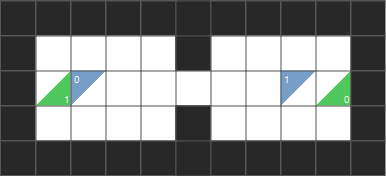
\includegraphics[height=40mm]{images/one_slit.png}
    \centering
    \caption{Aufbau für das Durchfahren zweier Agenten durch eine kurze Engstelle}
    \label{fig:engstelle}
\end{figure}
Die Karte misst neun mal drei Felder. In der Mitte der Karte ist eine eins mal eins Feld breite Engstelle. Auf beiden Seiten dieser Engstelle stehen sich Agenten gegenüber, die die Engstelle durchfahren müssen, um ihre Zielposition zu erreichen.

\textbf{Erwartete Beobachtungen}\newline
Der Agent, der zuerst einen Weg plant, fährt direkt auf seine Zielposition. Der andere Agent fährt eine Ausweichposition in der unmittelbaren Nähe der Engstelle an. Nachdem der erste Agent die Engstelle passiert hat, wird sich der zweite Agent auf direkten Weg zu seinem Ziel machen.
%
\subsection{Umweg}
\label{chap:umweg}
Hier wird gezeigt wie ein Agent einen anderen verdrängt, aber auch das Agenten Umwege in Kauf nehmen.

\textbf{Aufbau des Experiments}
\begin{figure}[H]
    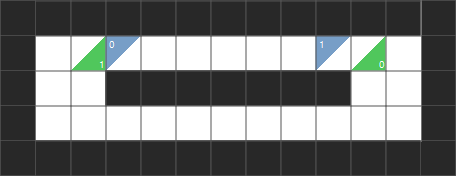
\includegraphics[height=40mm]{images/detour.png}
    \centering
    \caption{Aufbau für ein Szenario, in dem ein Agent einen Umweg in Kauf nimmt}
    \label{fig:umweg}
\end{figure}
Die Karte in Abbildung \ref{fig:umweg} misst elf mal drei Felder und wird mittig, horizontal durch einen Streifen aus sieben Feldern getrennt. Die Start- und Zielpositionen der Agenten sind so angeordnet, dass die nördliche Engstelle den kürzeren Weg darstellt und die südliche Engstelle den Umweg.

\textbf{Erwartete Beobachtungen}\newline
Für kleine Umgebungskarten, also solche bei denen sich die Umgebungskarten der beiden Agenten erst nach dem Annähern überlappen, werden sich beide Agenten in der nördlichen Engstelle annähern. Wenn sich die Umgebungskarten dann überlappen, wird einer der Agenten den Zuschlag erhalten und den anderen Agenten verdrängen. Dieser wird dann über die südliche Engstelle, also über den Umweg, sein Ziel anfahren.

Für größere Umgebungskarten wird der Agent, der zuerst seinen Weg plant, direkt und der andere über den Umweg sein Ziel anfahren.
%
\subsection{Tunnel}
\label{chap:tunnel}
Dieses Experiment testet, wie anfällig die Agenten für Verklemmungen sind.

\textbf{Aufbau des Experiments}
\begin{figure}[H]
    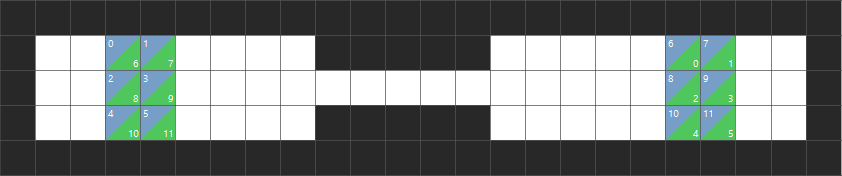
\includegraphics[width=\textwidth]{images/tunnel_2_groups.png}
    \centering
    \caption{Ausgangssituation für das Durchqueren eines Tunnels von zwei Gruppen, bestehend aus jeweils sechs Agenten}
    \label{fig:tunnel}
\end{figure}
In diesem Experiment durchqueren zwei Gruppen aus jeweils sechs Agenten eine Engstelle, die fünf Felder lang und ein Feld breit ist. Jeder Agent muss die Engstelle passieren um sein Ziel zu erreichen.

\textbf{Erwartete Beobachtungen}\newline
Im ersten Schritt nähern sich beide Gruppen der Engstelle. Während eine Gruppe anfängt die Engstelle zu durchqueren, fahren die Agenten der anderen Gruppe Ausweichpositionen an und verlängern damit die Engstelle. Im Laufe des Experiments wechseln die Gruppen ihre Rollen häufiger.
%
\subsection{Tunnel mit kleiner Ausweichbucht}
\label{chap:ausweichbucht}
Dieses Experiment dient zur Veranschaulichung der dynamischen Prioritäten. Diese Situation kann, dezentral, nämlich nicht durch feste Prioritäten gelöst werden.

\textbf{Aufbau des Experiments}
\begin{figure}[H]
    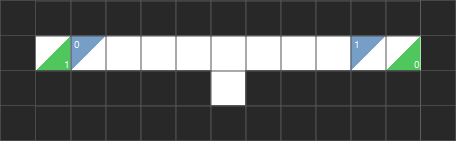
\includegraphics[height=32mm]{images/tunnel_turnout.png}
    \centering
    \caption{Aufbau für die Vorbeifahrt zweier Agenten in einem Tunnel mit einer kleinen Ausweichbucht}
    \label{fig:ausweichbucht}
\end{figure}
Zwei sich gegenüberstehende Agenten versuchen, in einer elf Felder langen und ein Feld schmalen Engstelle aneinander vorbei auf ihre Zielpositionen zu fahren. Der Tunnel hat in der Mitte ein zusätzliches freies Feld, das von den Agenten genutzt werden muss, um aneinander vorbei zu fahren.

\textbf{Erwartete Beobachtungen}\newline
Zuerst werden die beiden Agenten aufeinander zu fahren. Dann wird einer der beiden Agenten zurückgedrängt werden. Wenn der zurückgedrängte Agent sich nicht weiter zurückdrängen lässt, wird dieser seine Priorität erhöhen und den zu erst drängenden Agenten in die Ausweichbucht drängen, was dann beiden Agenten ermöglicht aneinander vorbei zu ihren Zielpositionen zu fahren. Es kann auch passieren, dass ein Agent die Ausweichbucht direkt anfährt und es zu keiner Verdrängung kommt.
%
\subsection{Durchfahren einer stehenden Menge}
\label{chap:menge}
In diesem Experiment wird gezeigt, dass obwohl ein Agent sein Ziel schon erreicht hat, immer noch aktiv an der passiven Kooperation teilnimmt.

\textbf{Aufbau des Experiments}
\begin{figure}[H]
    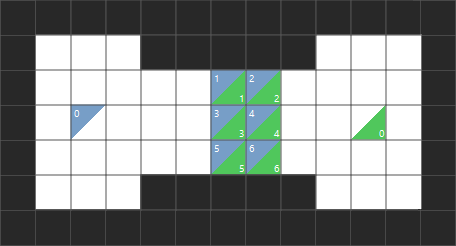
\includegraphics[height=56mm]{images/crowd_drive-through.png}
    \centering
    \caption{Aufbau für das Durchfahren eines Agenten durch ein Menge stehender Agenten}
    \label{fig:menge}
\end{figure}
Die Abbildung \ref{fig:menge} zeigt die Karte für dieses Experiment. Diese hat Dimensionen von elf mal fünf Felder. In der Mitte ist eine fünf Felder lange und drei Felder breite Engstelle. In dieser Engstelle stehen in zwei Reihen hintereinander sechs Agenten. Die Startpositionen dieser Agenten sind gleichzeitig ihre Zielpositionen. Ein weiterer Agent hat seine Startposition auf der linken Seite der Engstelle und seine Zielposition auf der Rechten. Er muss also durch die stehende Menge, um sein Ziel zu erreichen.

\textbf{Erwartete Beobachtungen}\newline
Die Agenten "'3"' und "'4"' werden von Agent "'0"' verdrängt, fahren also von ihren Zielpositionen weg, um Platz für Agent "'0"' zu machen. Es ist auch möglich, dass dabei andere Agenten von ihren Zielpositionen verdrängt werden. Nachdem Agent "'0"' die Menge durchquert hat, fahren alle Agenten wieder zurück zu ihren Zielpositionen.
%
\subsection{Kreuzung}
\label{chap:kreuzung}
Dieses Szenario dient der Beobachtung der Flexibilität der Agenten. Außerdem soll der Unterschied zu einem zentralen Ansatz deutlich gemacht werden und die Skalierbarkeit des Ansatzes gezeigt werden.

\textbf{Aufbau des Experiments}
\begin{figure}[H]
    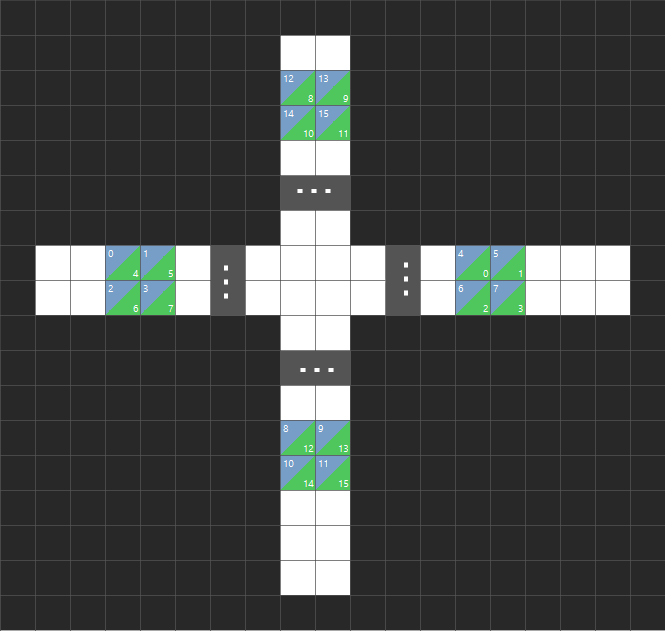
\includegraphics[width=\textwidth]{images/junction.png}
    \centering
    \caption{Aufbau für das Passieren einer Kreuzung von vier Gruppen, bestehend aus jeweils vier Agenten}
    \label{fig:kreuzung}
\end{figure}
In diesem Experiment versuchen vier Gruppen von jeweils vier Agenten eine Kreuzung zu durchqueren. Ziel jeder Gruppe ist es, die gegenüberliegende Seite in gleicher Formation zu erreichen. Der Kreuzungsbereich besteht aus acht freien Feldern, bietet also nicht genügend Platz für alle Agenten. Normale Verkehrsregeln, zum Beispiel das Rechtsfahrgebot, Vorfahrtsregeln oder das Bilden von Fahrspuren, sind keine Lösungen, die ein konfliktfreies aneinander Vorbeifahren der Agenten ermöglichen. Die vier Fahrbahnen der Kreuzung sind jeweils zwei Felder breit und 14 Felder lang.

\textbf{Erwartete Beobachtungen}\newline
Wegen der dynamischem Prioritäten ist eine Vielzahl an Lösungen zu beobachten. Der Berechnungsaufwand pro Agent steigt, trotz der gestiegenen Teilnehmerzahl, nicht.
Ein möglicher zentraler Ansatz würde vermutlich zwei Gruppen blockieren und die übrigen gegenüberliegenden Gruppen durch die Kreuzung passieren lassen, um erst danach den blockierten Gruppen die Durchfahrt zu gewähren. Dies ist vergleichbar mit einer Ampel an einer Kreuzung im Straßenverkehr.


%
\subsection{Beobachtungen}
\label{chap:beobachtungen}
Alle zu erwartenden Beobachtungen konnten, so wie in \cite{book:regele} beschrieben, in den eigens ausgeführten Experimenten beobachtet werden.

\section{Experimente mit Messwerten}
\label{chap:mitMesswerten}
Die folgenden Experimente wurden zum Überprüfen der Leistungsfähigkeit des Algorithmus entwickelt. Im Kern stehen sich immer zwei gleich große Gruppen von Agenten gegenüber, deren Ziel es ist die Startpositionen der Agenten der anderen Gruppen zu erreichen. Die Anzahl der Agenten variiert zwischen den Experimenten und der freie Raum wird tendenziell immer kleiner. Für jedes Experiment ist es das Ziel, dass in allen 30 Wiederholung eine Lösung gefunden wird, also alle Agenten ihr Ziel erreichen.

Der Aufbau der Experimente und das zu erwartende Verhalten der Agenten werden vorgestellt. Im Kapitel \ref{chap:ergebnisse} folgen dann die Messwerte aus \cite{book:regele} und die eigenen.

\subsection{Sechs gegen sechs: Lockere Vorbeifahrt}
\label{chap:6x6_locker}
Das erste Experiment dieser Reihe bietet vergleichsweise viel Platz. Es ist vor allem für den späteren Vergleich interessant.

\textbf{Aufbau des Experiments}
\begin{figure}[H]
    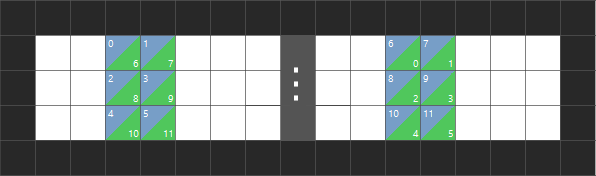
\includegraphics[width=\textwidth]{images/6vs6_spacy.png}
    \centering
    \caption{Aufbau für die lockere Vorbeifahrt zweier Gruppen, bestehend aus jeweils sechs Agenten}
    \label{fig:6x6Locker}
\end{figure}
 Die Abbildung \ref{fig:6x6Locker} zeigt eine Karte die drei mal 30 Felder misst. Es stehen sich zwei Gruppen, bestehend aus jeweils sechs Agenten, gegenüber. Zum rechten beziehungsweise linken Rand sind für die Gruppen noch ein paar freie Felder vorhanden. Damit soll es den Agenten möglich sein, Ausweichbewegungen nach hinten hin ausführen zu können.
\subsection{Sechs gegen sechs: Enge Vorbeifahrt}
\label{chap:6x6_eng}
In diesem Experiment ist der Platz für Bewegungen sehr beschränkt. Zwölf Felder sind von Agenten belegt und lediglich neun sind frei. 

\textbf{Aufbau des Experiments}
\begin{figure}[H]
    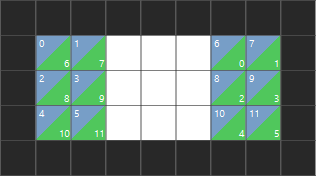
\includegraphics[height=40mm]{images/6vs6_tight.png}
    \centering
    \caption{Aufbau für die enge Vorbeifahrt zweier Gruppen, bestehend aus jeweils sechs Agenten}
    \label{fig:6x6Eng}
\end{figure}
Die Karte für dieses Experiment ist sieben mal drei Felder groß. Es stehen sich zwei Gruppen aus jeweils sechs Agenten gegenüber. Wie in Abbildung \ref{fig:6x6Eng} zu erkennen, befindet sich zwischen den beiden Gruppen ein Block aus drei mal drei freien Feldern.
\subsection{Drei gegen drei: Enge Vorbeifahrt}
\label{chap:3x3_eng}
Dieses Experiment dient als Vergleich zum Vorangegangenen. Die Auswirkung die die Anzahl der Roboter hat, soll hiermit untersucht werden. 

\textbf{Aufbau des Experiments}
\begin{figure}[H]
    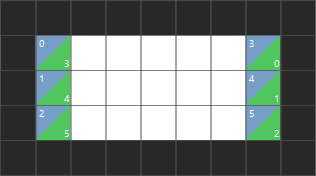
\includegraphics[height=40mm]{images/3vs3.png}
    \centering
    \caption{Aufbau für die enge Vorbeifahrt zweier Gruppen, bestehend aus jeweils drei Agenten}
    \label{fig:3x3}
\end{figure}
Die Karte für dieses Experiment ist sieben mal drei Felder groß. Es stehen sich zwei Gruppen aus jeweils drei Agenten gegenüber. Wie in Abbildung \ref{fig:3x3} zu erkennen, befindet sich zwischen den beiden Gruppen ein Block aus fünf mal drei freien Feldern.
\subsection{Vier gegen vier: Enge Vorbeifahrt}
\label{chap:4x4_eng}
Dieses Experiment schränkt den Platz der Agenten weiter ein. Die Zahl der belegten Felder ist hier größer als die Anzahl der freien Felder. Besonders für dieses Experiment ist, dass ein Graph vorliegt der die Prioritätswerte der Agenten über die Zeit zeigt (siehe Abbildung \ref{tab:resultsCoDy} und \ref{tab:myResults}). 

\textbf{Aufbau des Experiments}
\begin{figure}[H]
    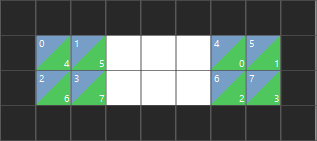
\includegraphics[height=32mm]{images/4vs4_tight.png}
    \centering
    \caption{Aufbau für die enge Vorbeifahrt zweier Gruppen, bestehend aus jeweils vier Agenten}
    \label{fig:4x4}
\end{figure}
Die Karte für dieses Experiment misst sieben mal zwei Felder. Acht Agenten teilen sich in zwei gleich große Gruppen und stehen sich gegenüber.
\subsection{Messergebnisse}
\label{chap:ergebnisse}
\begin{table}[H]
    \centering
    \begin{tabular}{c|c|c|c|c|c|c}
       \textbf{Experiment} & \textbf{Gelöst} & \textbf{Prioritäts-Überlauf}
        & \(\textbf{s\textsubscript{opt}}\) & \(\textbf{s\textsubscript{CoDy}}\)
        & \(\textbf{t\textsubscript{opt}}\) & \(\textbf{t\textsubscript{CoDy}}\)\\ \hline
       \textbf{6-vs-6-locker} & 30 von 30 & 0 von 30
       & 19.5 & 20.97 & 22 & 24.33 \\ \hline
       \textbf{6-vs-6-eng} & 26 von 30 & 1 von 30
       & 5.45 & 11.5 & 10.35 & 21.89 \\ \hline
       \textbf{3-vs-3-eng} & 30 von 30 & 3 von 30
       & 5.5 & 6.35 & 6.33 & 7.68 \\ \hline
       \textbf{4-vs-4-eng} & 27 von 30 & 4 von 30
       & 5 & 10.85 & 10.5 & 24.96
    \end{tabular}
    \caption{Messwerte der Experimente aus \cite{book:regele}}
    \label{tab:resultsCoDy}
\end{table}

\begin{table}[H]
    \centering
    \begin{tabular}{c|c|c|c|c}
       \textbf{Experiment} & \textbf{Gelöst} & \textbf{Prioritäts-Überlauf}
        & [\textbf{\(\bar{s}\textsubscript{u}\)}, \textbf{\(\bar{s}\textsubscript{o}\)}]
        & [\textbf{\(\bar{t}\textsubscript{u}\)}, \textbf{\(\bar{t}\textsubscript{o}\)}]\\ \hline
       \textbf{6-vs-6-locker} & 30 von 30 & 0 von 30 & [20.01, 22.33] & [23.92, 26.4]\\ \hline
       \textbf{6-vs-6-eng} & 18 von 30 & 18 von 18 & [8.78, 9.81] & [19.52, 23.09]\\ \hline
       \textbf{3-vs-3-eng} & 27 von 30 & 0 von 27 & [7.3, 7.58] & [9.53, 9.97]\\ \hline
       \textbf{4-vs-4-eng} & 20 von 30 & 20 von 20 & [13.72, 25.2] & [23.04, 41.04]
    \end{tabular}
    \caption{Messwerte der selbst durchgeführten Experimente}
    \label{tab:myResults}
\end{table}

Die eigenen Messwerte weichen teils stark von den vorgegeben Messwerten ab. Lediglich das Experiment "'\ref{chap:6x6_locker} Sechs gegen sechs: Lockere Vorbeifahrt"' trifft die Erwartungen.

Für die eigenen Messungen ist anzumerken, dass für den Prioritätsüberlauf nicht immer "'von 30"' angegeben ist. Das hat damit zu tun, dass die Simulationsumgebung nur Daten erzeugt, wenn ein Experiment erfolgreich war.

\begin{figure}[H]
    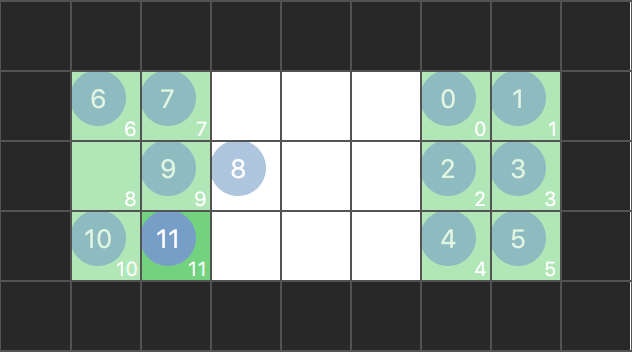
\includegraphics[height=40mm]{images/6vs6_tight_full_block.png}
    \centering
    \caption{Beispielhafte Totalblockade für das Experiment "'\ref{chap:6x6_eng} Sechs gegen sechs: Enge Vorbeifahrt"'}
    \label{fig:6x6EngFullBlock}
\end{figure}
Für das Experiment "'\ref{chap:6x6_eng} Sechs gegen sechs: Enge Vorbeifahrt"' ist der zurückgelegte Strecke etwas besser als erwartet. Der Zeitbedarf trifft die Erwartung. Auffällig ist jedoch, dass nur 18 statt 26 Wiederholungen erfolgreich sind und es in allen, statt nur bei einer Wiederholung, zu Prioritätsüberläufen kam. Bei den zwölf ungelösten Wiederholungen ist eine Variation der in Abbildung \ref{fig:6x6EngFullBlock} gezeigten Situation eingetreten. 

Die Werte für "'\ref{chap:3x3_eng} Drei gegen drei: Enge Vorbeifahrt"'
weichen nur leicht von den erwarteten ab. Statt 30 werden nur 27 Wiederholungen gelöst. Dafür kommt es in den gelösten Wiederholungen aber nicht zu Prioritätsüberläufen. Die drei erwarteten Wiederholungen, die einen Prioritätsüberläufen haben, entstehen aus Situationen, in denen sich die Agenten in breiter Front aufeinander zu bewegen. In den eigenen Experimenten führten genau diese Situation zu den drei ungelösten Wiederholungen.

Die gemessenen Werte weichen für das Experiment "'\ref{chap:4x4_eng} Vier gegen vier: Enge Vorbeifahrt"' am stärksten ab. Es werden nur in 20 statt 27 Wiederholungen Lösungen gefunden. In jeder Wiederholung kommt es zu Prioritätsüberläufen. Auch das war nicht erwartet. Die Konfidenzintervalle für die durchschnittlich zurückgelegte Strecke und den durchschnittlichen Zeitbedarf sind im Vergleich besonders groß. Die erwartete Strecke ist nicht mal im Intervall enthalten. Wie Abbildungen \ref{fig:4x4_prio_2} deutlich zeigt, wird der erwartete Prioritätsverlauf verfehlt. Statt das die Priorität der Agenten über die Zeit stetig ansteigt und teilweise wieder zurückgeht, pendeln bei den eigenen Experimenten die Prioritätswerte zwischen minimalen und maximalen Werten hin und her.

\begin{figure}[H]
    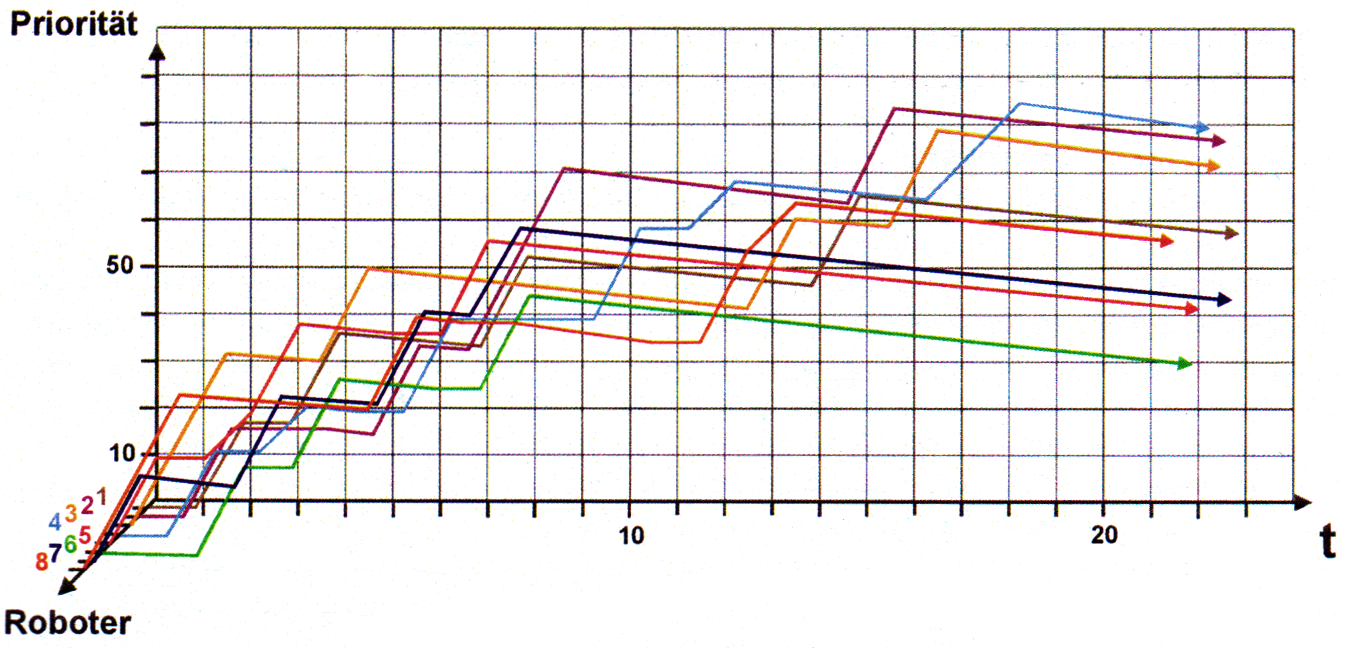
\includegraphics[width=\textwidth]{images/4vs4_tight_prio_ref.png}
    \centering
    \caption{Prioritätsverlauf aller Agenten für das Experiment "'\ref{chap:4x4_eng} Vier gegen vier: Enge Vorbeifahrt"' aus \cite{book:regele}}
    \label{fig:4x4_prio_1}
\end{figure}

\begin{figure}[H]
    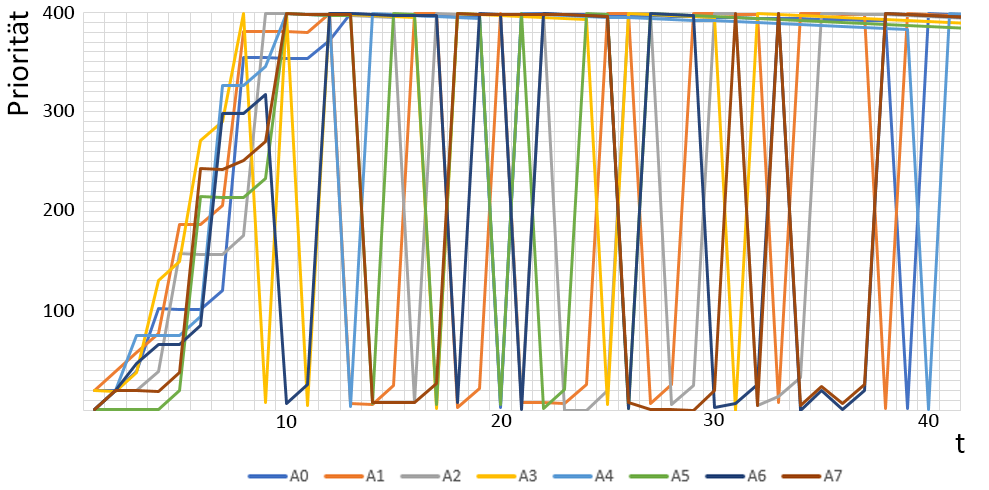
\includegraphics[width=\textwidth]{images/4vs4_tight_prio.png}
    \centering
    \caption{Prioritätsverlauf aller Agenten für das Experiment "'\ref{chap:4x4_eng} Vier gegen vier: Enge Vorbeifahrt"' der selbst durchgeführten Experimente}
    \label{fig:4x4_prio_2}
\end{figure}
%
\chapter{Diskussion}
\label{chap:diskussion}
Gerade im Rahmen der Programmierlehre scheint der Einsatz von CRS relativ sinnvoll zu sein, denn der Umgang mit Programmiersprachen lässt sich gut objektiv bewerten und leicht in Fragen fassen. Dennoch gibt es bei bestehenden CRS häufig große Hürden, um sie im Kontext der Programmierlehre einzusetzen. Deswegen werden hier zwei bestehende CRS aus dem akademischen Bereich miteinander verglichen: Einerseits die bisher an der HAW Hamburg eingesetzte Lösung StuReSy und zum Vergleich eine populäre, kommerziellere Lösung namens Pingo.

\section{StuReSy}
\label{chap:sturesy}
\ac{sturesy} ist der Name einer Software, die im Rahmen der Bachelorarbeit von Wolf Posdorfer im Jahr 20012 an der Universität Hamburg entstanden ist. Der Name StuReSy ist ein Akronym für „Student Response System“.

StuReSy besteht aus zwei Komponenten:
\begin{itemize}
    \item Server-Komponente: In PHP geschrieben, agiert gleichzeitig auch als Client-Komponente für die Abstimmungs-Teilenehmer. Inkludiert eine relationale SQL-Datenbank.
    \item Admin-Komponente: Um Fragen zu erstellen und zu bearbeiten wird ein Client als Java-Anwendung benötigt.
\end{itemize}

StuReSy wurde erfolgreich und viele Jahre an der Universität Hamburg und HAW Hamburg eingesetzt. Die Qualität und der Umfang der Software sind für eine Bachelorarbeit beeindruckend.

Dennoch verfügt StuReSy über einige Nachteile und Probleme:
\begin{itemize}
    \item Software-Download und JVM notwendig: Um StuReSy administrativ einsetzen zu können, muss eine Java-Software heruntergeladen werden und eine JVM muss auf dem jeweiligen System vorhanden sein. Eine Administration vom Tablet oder Smartphone ist damit nur schwer möglich.
    \item Server-Komponente: Um StuReSy betreiben zu können, wird eine Server-Instanz benötigt. Diese muss von der jeweiligen Institution oder einem Dozenten aufgesetzt und gewartet werden.
    \item Mangelnde Formatierungsmöglichkeiten für Software-Quelltext: In der Praxis wird StuReSy vor allem in Informatik-Veranstaltungen eingesetzt. Dort werden oft Fragen zu Quelltexten gestellt. Die Darstellung dieser Quelltexte ist schwierig: Zentrierte Text-Ausrichtung .... sorgen für unübersichtliche Darstellung.
\end{itemize}


\newpage
\section{Pingo}
\label{chap:pingo}
Pingo ist eine Software-Lösung, die bereits seit dem Jahr 2011 an der Universität Paderborn entwickelt wird. Der Name ist ebenfalls ein Akronym und steht für „\textbf{P}eer \textbf{In}struction for Very Large \textbf{G}r\textbf{o}ups“. Im Gegensatz zu StuReSy ist Pingo bereits weiter verbreitet und wird an vielen deutschen Hochschulen eingesetzt. Dahinter steht außerdem ein ganzes Team von akademischen Mitarbeitern. Seit 2019 wird Pingo von der universitätsnahen Coactum GmbH betrieben und weiterentwickelt.\newline

Prinzipiell handelt es sich bei Pingo um eine reine Web-Applikation, die öffentlich und kostenlos unter www.trypingo.com zugänglich ist. Für die Nutzung muss jedoch ein Benutzerkonto eröffnet werden. Pingo steht unter einer Open-Source-Lizenz und somit können Nutzer auch eine eigene Pingo-Instanz betreiben. Pingo ist in der Programmiersprache Ruby und mithilfe des Web-Frameworks „Ruby on Rails“ implementiert worden.

Bei den unterstützten Fragetypen sind beide Programme nahezu identisch: Single Choice, Multiple Choice, Freitext und numerische Fragen sind möglich.


Pingo hat prinzipiell einen sehr großen Funktionsumfang, jedoch fehlen entscheidende Funktionen für den Einsatz in der Programmierlehre:
\begin{itemize}
    \item \textbf{Keinerlei Formatierungs-Möglichkeiten}: Fragen innerhalb der Pingo-Plattform können überhaupt nicht formatiert werden. Damit können weder Fettschreibungen, Unterstreichungen oder Zeilenumbrüche verwendet werden. Dementsprechend ist auch die übersichtliche Darstellung von Quelltext vollkommen unmöglich.
\end{itemize}

\begin{figure}[H]
    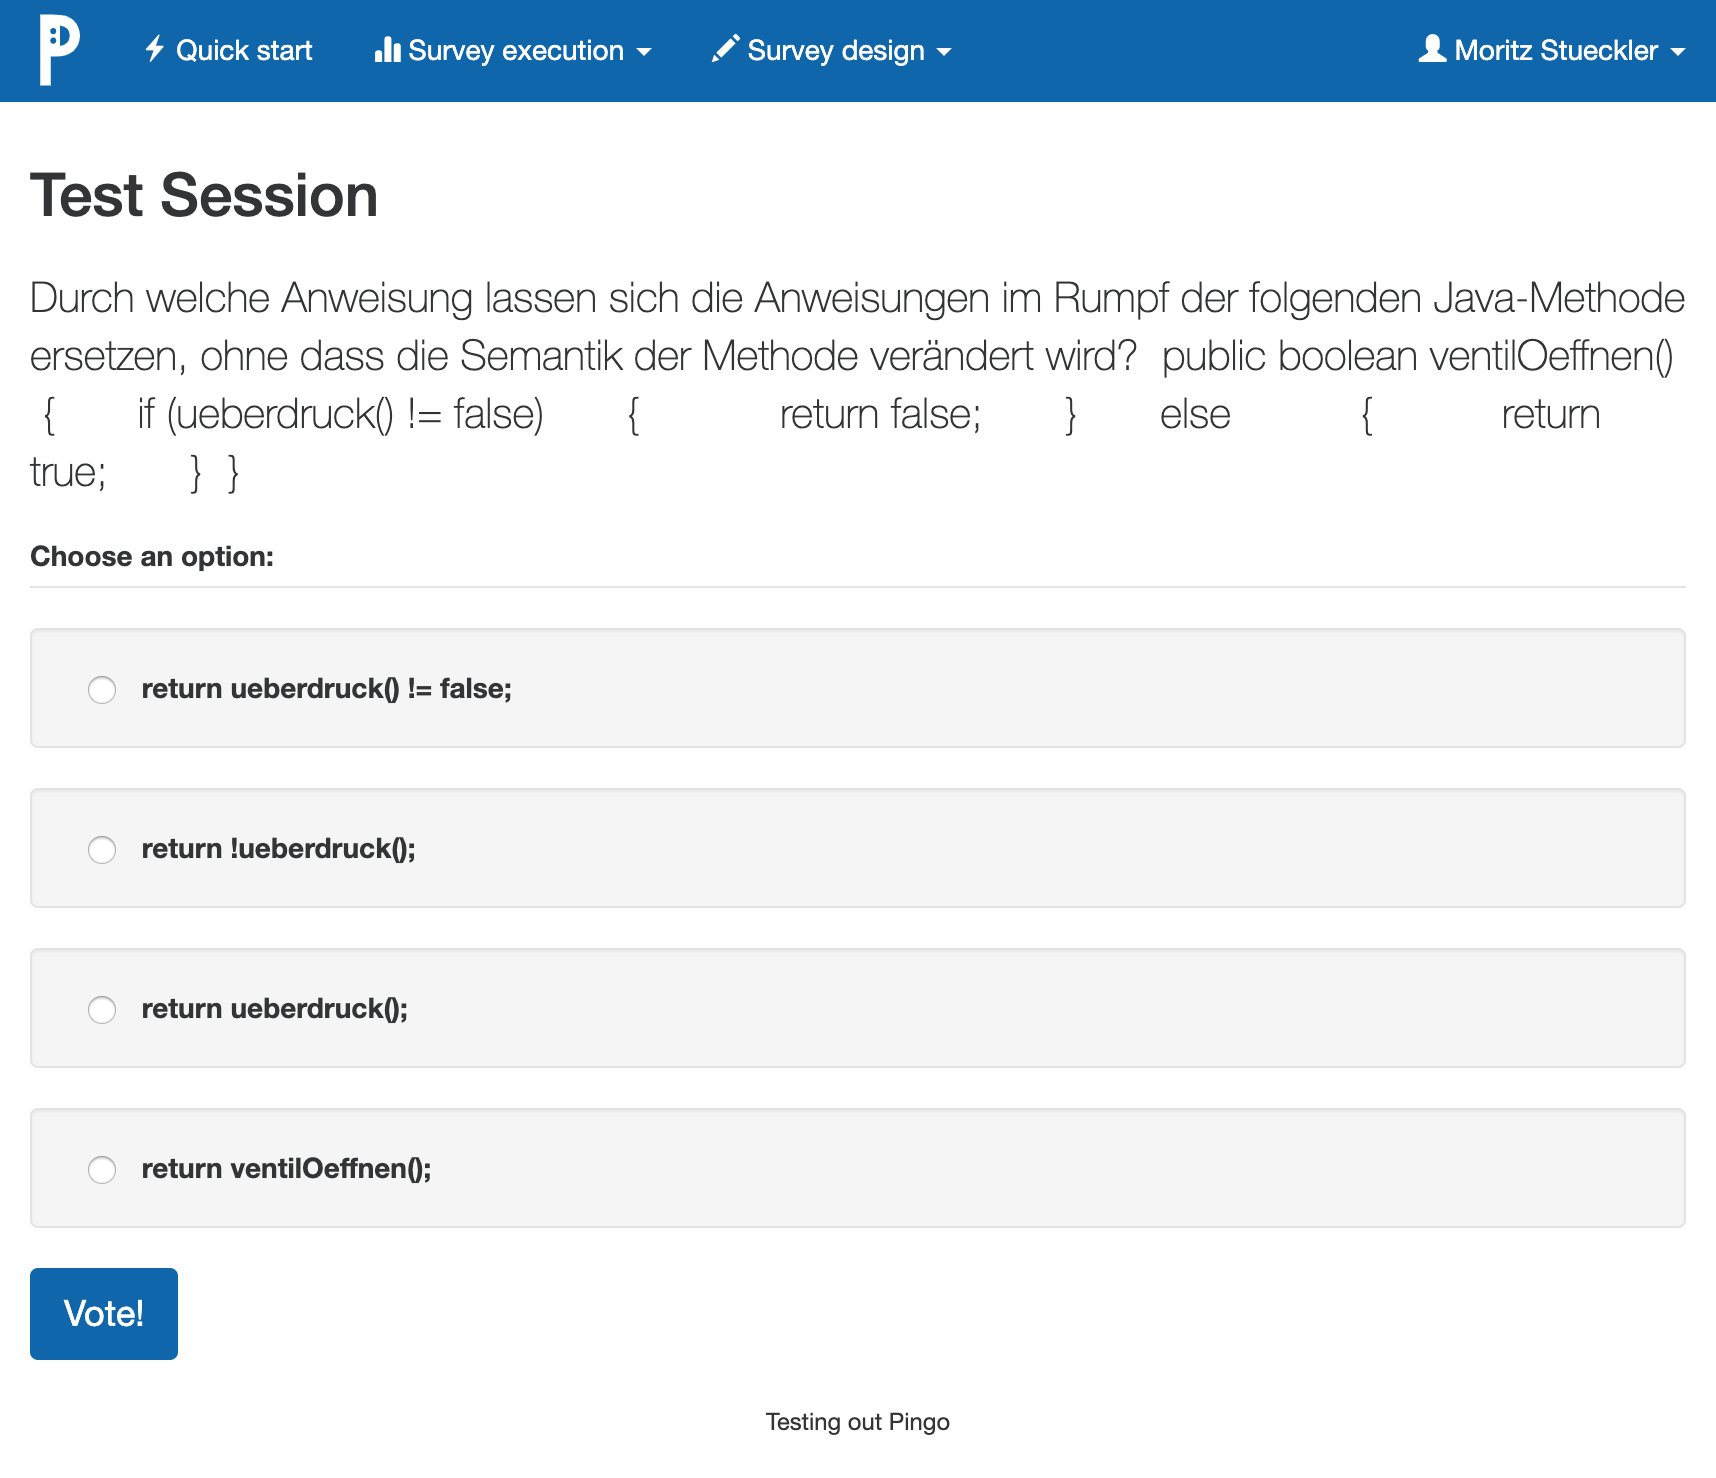
\includegraphics[width=12cm]{chapter/bewertung/bilder/pingo_problem1.png}
    \centering
    \caption{Pingo verfügt über keinerlei Text-Formatierungsoptionen und ist daher ungeeignet für die Darstellung von Quelltext.}
    \label{Abbildung 2.4}
\end{figure}
%
\chapter{Fazit}
\label{chap:fazit}
Für jede der ermittelten Anforderungen soll einzeln erörtert werden, ob die Umsetzung gelungen ist, und welche Erfahrungen bei der Implementierung gemacht werden konnten.

\subsubsection*{Web-Applikation}
Trotz einiger Nachteile, die der Browser als Laufzeitumgebung mit sich bringt, erscheint es sinnvoll und zeitgemäß, ein CRS vollständig webbasiert zu implementieren. Die technischen Anforderungen an das ausführende System sind relativ gering. Die Anforderungen an die User Experience und eine gut gestaltete Benutzeroberfläche im Gegensatz dazu eher hoch. Es erscheint daher nicht mehr zeitgemäß für die technisch relativ simple Aufgabe, die ein CRS bewältigt, Software extra herunterladen und installieren zu müssen (es sei denn es gibt Gründe wie etwa geforderte Hardware-Kompatibilität).

Das React-Framework hat sich als gute Wahl für diese Aufgabe herausgestellt. Die bereitgestellten Konzepte und Bibliotheken waren relativ einfach zu verstehen und haben eine sehr schnelle Entwicklung ermöglicht. Langfristige Wartbarkeit scheint durch die Größe der React-Gemeinde ebenfalls gegeben zu sein.

Eine wichtige Erfahrung dieser Arbeit war der Umgang mit dem enorm großen JavaScript-Ökosystem. Zwar ist die Masse an verfügbaren und kostenlosen, OpenSource-JavaScript-Bibliotheken überwältigend, allerdings zeigt sich, dass es oft schwer ist, stabile und zuverlässige Projekte zu finden. Die Anzahl und Aktivität der Entwickler sowie die Häufigkeit von Updates waren oftmals bessere Kriterien für die Auswahl einer Bibliothek als ihr anfänglicher Funktionsumfang.

\subsubsection*{Peer-To-Peer-Verbindungen}
Die Implementierung von Peer-to-Peer-Verbindungen auf Basis von WebRTC erwies sich als schwierig. Der WebRTC-Standard ist leider noch nicht fertiggestellt, und die Abweichungen zwischen den Implementierungen der verschiedenen Browser-Hersteller sind relativ groß. WebRTC im Produktiveinsatz mit breiter Kompatibilität zu verwenden ist aufwändig, das scheinen auch große Firmen zu sehen: Erst kürzlich aktualisierte Microsoft seinen „Skype for Web“-Dienst mit WebRTC-Technologie. Zunächst wurden dabei alle anderen Browser außer Google Chrome ausgesperrt – vermutlich ist die schwierige WebRTC-Kompatibilität einer der Gründe dafür\footnote{Quelle: \url{https://arstechnica.com/gadgets/2019/03/microsofts-new-skype-for-web-client-an-early-taste-of-the-browser-monoculture/}}.

Die Verwendung von WebRTC-Wrappern wie PeerJS, die die Schnittstelle vereinfachen und das Signalling regeln, erscheint gerade in kleinen Projekten daher unausweichlich zu sein. Leider gibt es bisher nicht sehr viele, und nicht sehr aktuelle Open-Source-Bibliotheken für diese Aufgabe. Es bleibt zu hoffen dass die Stabilität der Schnittstelle und damit auch die Qualität der Wrapper-Bibliotheken nach dem Ende der WebRTC-Standardisierung ein besseres Niveau erreicht.

Das fertige System funktioniert zwar einwandfrei, allerdings kann es schnell zu Komplikationen kommen, zum Beispiel wenn die Verbindung der Teilnehmer während einer Sitzung unterbrochen wird oder wenn Browser-Versionen nicht unterstützt werden.

\subsubsection*{Code-Formatierung}
Die Einbindung von bestehenden, Editor-Bibliotheken war eine sehr gute Entscheidung. Es gibt eine große Anzahl von sehr aktiven JavaScript-Editor-Bibliotheken, allerdings bieten nur wenige davon auch eine überzeugende React-Integration an.

\subsubsection*{Code-Ausführung im Browser}
Weclare zeigt, dass die Ausführung von Java-Quellcode im Browser grundsätzlich möglich ist. Wie praktikabel dieses Experiment im Alltag der Dozenten ist bleibt fraglich. Vor allem das notwendige Laden der Java-Runtime sorgt dafür dass die Ausführungsdauer von Code-Beispielen oft unangenehm lange ist. Bei geladener Runtime können Code-Beispiele meistens innerhalb von 15 bis 30 Sekunden kompiliert und ausgeführt werden. Je nach Geschwindigkeit der Internetverbindung kann sich dieser Wert beim ersten Laden der Runtime auf mehrere Minuten vergrößern.

Probleme:
\begin{itemize}
    \item Unit- und Integrationstest für die Anwendung sind dringend notwendig
    \item Die Instantiierung der DoppioJVM sollte in einem eigenen Thread erfolgen und deswegen in einen WebWorker ausgelagert werden
    \item Freitext-Fragen, wie sie von StuReSy und Doppio unterstützt werden, sind nicht implementiert
    \item Die Visualisierung der erhaltenen Antworten in Form von Diagrammen und der Export als Grafik oder CSV wird nicht unterstützt
\end{itemize}





%%%%%% Chapters End

%% bibliography and other stuff
\backmatter

\typeout{===== Section: literature}
%% read the documentation for customizing the style
\printbibliography
\typeout{===== Section: nomenclature}
%% uncomment if a TOC entry is needed
%% \addcontentsline{toc}{chapter}{Glossar}
\renewcommand{\nomname}{Glossar}
\clearpage
\markboth{\nomname}{\nomname} %% see nomencl doc, page 9, section 4.1
\printnomenclature

%% index
\typeout{===== Section: index}
\printindex

\HAWasurency

\end{document}
